\renewcommand*{\chapter}{\OrigChapter}
\vspace{3.0ex}
\footnotesize
\uppercase{1. Siglen und editorische Zeichen}\\[1.0ex]
\begin{tabular}{lp{110mm}}
\textit{E} & Erstdruck\\
\textit{E}\textsuperscript{1}, \textit{E}\textsuperscript{2} & weitere Drucke\\
\textit{L} & Leibniz, eigenh\"{a}ndig\\
\textit{l} & Leibniz, Abschrift von Schreiberhand\\
\textit{A} & Abschrift eines fremden Textes\\
\textit{LiH} & Leibniz' eigenh\"{a}ndige Bemerkungen in einem Handexemplar\\
\textit{Lil} & Leibniz' Korrekturen zu einer Abschrift von Schreiberhand\\
\textit{LiA} & Leibniz' Bemerkungen und Korrekturen in der Abschrift eines fremden Textes\\
$[~]$ & in der Datierung: erschlossenes Datum\newline im Text: Erg\"{a}nzungen des Herausgebers\newline von Leibniz gelegentlich benutzte eckige Klammern werden im Erl\"{a}uterungs\-apparat angezeigt\\
\textit{[~]} & vom Herausgeber hinzugef\"{u}gte Figurenbezeichnungen\\
\textit{(~)} & von Leibniz in Figuren seines Handexemplars hinzugef\"{u}gte Bezeichnungen\\
$\langle$\ $\rangle$ & Konjektur schwer lesbarer oder durch Besch\"{a}digung des Textzeugen ausgefallener W\"{o}rter bzw. Wortteile\\
$\langle$\textendash $\rangle$~$\langle$\textendash \textendash$\rangle$ & nicht entziffertes bzw. durch Besch\"{a}digung aus\-gefallenes Wort; die Anzahl der Striche entspricht der Anzahl der vermuteten W\"{o}rter.\\
\textit{Kursivierung} & w\"{o}rtliche oder fast w\"{o}rtliche Zitate, Buchtitel, vom Herausgeber hinzugef\"{u}gter Text. Fast w\"{o}rtlich meint geringf\"{u}gige Abweichungen ohne Signifikanz wie fl\"{u}chtige Wiedergaben der Wortfolge oder Kasus\"{a}nderungen durch Leibniz.\\
\textso{Sperrung} & Hervorhebungen von Leibniz. Die Art der Hervorhebung wird im Er\-l\"{a}uterungsapparat angezeigt.
\end{tabular}
\vspace{2.0ex}

\noindent\footnotesize{\uppercase{2. Abk\"{u}rzungen} (allgemein)}
\setlength\LTleft{0pt} \setlength\LTright{0pt}
\begin{longtable}{ll}
\footnotesize
a.a.O. & am angegebenen Ort\\
Anm. & Anmerkung\\
Aufl. & Auflage\\
Bd(e) & Band (B\"{a}nde)\\
Bl. & Blatt\\
Bog. & Bogen\\
bzw.  & beziehungsweise\\
ca & circa\\
ebd. & ebenda\\
erg. & erg\"{a}nzt\\
Fig. & Figur\\
f. & folgend\\
ff. & folgende (pl.)\\
gestr. & gestrichen\\
Hrsg. (hrsg.) & Herausgeber (herausgegeben)\\
Jh. & Jahrhundert\\
k.E. & kein Eintrag\\
LBr & HANNOVER, \textit{Gottfried Wilhelm Leibniz-Bibliothek}, Leibniz-Briefwechsel\\
LH & HANNOVER, \textit{Gottfried Wilhelm Leibniz-Bibliothek}, Leibniz-Handschriften\\
Marg. & Marginalie(n)\\
Ms. & Manuskript\\
N., Nr. & Nummer\\
Nachdr. & Nachdruck\\
o. S. & ohne Seitenangabe\\
r\textsuperscript{o} & recto\\
RS & Royal Society\\
S. & Seite\\
s.a. & siehe auch\\
s.o. & siehe oben\\
s.u. & siehe unten\\
Sp. & Spalte\\
SV & Schriftenverzeichnis\\
TD & Teildruck\\
tlw. & teilweise\\
u.a. & und andere, unter anderem\\
v. & van, von\\
Var. & Variante\\
vgl. & vergleiche\\
vermutl. & vermutlich\\
v\textsuperscript{o} & verso\\
Z. & Zeile\\
\Denarius & destilletur, distilletur (noch zu bedenken)
\end{longtable}
\vspace{2.0ex}
%\clearpage
\noindent\footnotesize{\uppercase{3. Abk\"{u}rzungen} (Schriften)}\par
\vspace{1.0ex}
%\setlength\LTleft{0pt} \setlength\LTright{0pt}
%\begin{longtable}{lp{105mm}}
\noindent\hangindent=10mm\textit{BH}: \textsc{Birch, Th.}, \textit{The History of the Royal Society of London for improving of natural knowledge: from its first rise}, London 1757.\par
\noindent\hangindent=10mm\textit{BW}: \textsc{Boyle, R.}, \textit{The Works}, hrsg. von M. Hunter und E. B. Davis, London 1999ff.\par
\noindent\hangindent=10mm Cc 2: \textit{Catalogue critique des manuscrits de Leibniz, Fascicule  II (Mars 1672\textendash Novembre 1676)}, hrsg. von A. Rivaud u.a., Poitiers 1914\textendash 1924.\par
\noindent\hangindent=10mm\textit{DO}: \textsc{Descartes, R.}, \textit{Oeuvres}, hrsg. von Ch. Adam u. P. Tannery, 12 Bde, Paris 1879\textendash 1910, 2. Aufl. ebd. 1964\textendash 1972.\par
\noindent\hangindent=10mm\textsc{Dutens}: \textsc{Leibniz, G. W.}, \textit{Opera omnia, nunc primum collecta, in classes distributa, praefationibus et indicibus exornata}, hrsg. von L. Dutens, 6 Bde, Genf 1768, Nachdr. Hildesheim 1989.\par
\noindent\hangindent=10mm\textsc{Gerland} 1906: \textsc{Leibniz, G. W.}, \textit{Nachgelassene Schriften physikalischen, mechanischen und technischen Inhalts}, hrsg. von E. Gerland, Leipzig 1906, Nachdr.: Hildesheim, New York 1995.\par
\noindent\hangindent=10mm\textit{GO}: \textsc{Galilei, G.}, \textit{Le Opere}, Edizione Nazionale, hrsg. von A. Favaro u.a., 20 Bde, Florenz 1890\textendash 1909. Neuausgabe von S. Garbasso u. Mitarbeiter, Florenz 1929\textendash 1932.\par
\noindent\hangindent=10mm\textit{GOO}: \textsc{Gassendi, P.}, \textit{Opera omnia}, 6 Bde, Lyon 1658, Nachdr.: Stuttgart-Bad Cannstatt 1964.\par
\noindent\hangindent=10mm\textit{HO}: \textsc{Huygens, Chr.}, \textit{Oeuvres compl\`{e}tes}, hrsg. von D. Bierens de Haan, J. Bosscha u.a., 22 Bde, Den Haag 1888\textendash 1950.\par
\noindent\hangindent=10mm\textit{JS}: \textit{Journal des S\c{c}avans}, Paris 1665ff.\par
\noindent\hangindent=10mm\textit{KGW}: \textsc{Kepler, J.}, \textit{Gesammelte Werke}, hrsg. von der Bayerischen Akademie der Wissenschaften, M\"{u}nchen 1923ff.\par
\noindent\hangindent=10mm KK 1: \textit{Kritischer Katalog der Leibniz-Handschriften, 1. Heft 1646\textendash 1672}, hrsg. von P. Ritter, als Manuskript ver\"{o}ffentlicht Berlin 1908.\par
\noindent\hangindent=10mm\textit{LSB}: \textsc{Leibniz, G. W.}, \textit{S\"{a}mtliche Schriften und Briefe}, Akademie Ausgabe, Darmstadt 1923ff. (seit 1954: Berlin).\par
\noindent\hangindent=10mm\textit{PO}: \textsc{Pascal, B.},	\textit{Oeuvres}, hrsg. von P. Boutroux, L. Brunschvicg, F. Gazier, 14~Bde, Paris 1904\textendash 1914, Nachdr.: Vaduz 1965.\par
\noindent\hangindent=10mm\textit{PT}: \textit{Philosophical Transactions}, London 1665ff.\par
\noindent\hangindent=10mm\textit{SPW}: \textsc{Stevin, S.}, \textit{The principal works}, hrsg. von E. J. Dijksterhuis u.a., Amsterdam 1955\textendash 1966.\par
\noindent\hangindent=10mm\textit{TO}: \textsc{Torricelli, E.}, \textit{Opere}, hrsg. von G. Loria, G. Vassura, 4 Bde, Faenza 1919\textendash 1944.\par
\noindent\hangindent=10mm\textit{WO}: \textsc{Wallis, J.}, \textit{Opera mathematica}, 3 Bde, Oxford 1693\textendash 1699, Nachdr.: Hildesheim 1972.\par
%\end{longtable}
\vspace{3.0ex}

\noindent\footnotesize{\uppercase{4. Symbole und Zeichen}}
\setlength\LTleft{0pt} \setlength\LTright{0pt}
\begin{longtable}{lp{100mm}}
\footnotesize
\earth & Antimon\\
\saturn & Blei (Saturn)\\
\mars & Eisen (Mars)\\
\astrosun & Gold (Sonne)\\
\mercury & Quecksilber (Merkur)\\
\Pfund & Pfund\\
\rightmoon & Silber (Mond)\\
\jupiter & Zinn (Jupiter)\\
\protect
\includegraphics[width=0.02\textwidth]{images/vitriol.pdf} & Vitriol\\
\protect
\includegraphics[width=0.02\textwidth]{images/salpeter.pdf} & Salpeters\"{a}ure\\
\protect
\includegraphics[width=0.02\textwidth]{images/taros.pdf} & Weinstein\\
$\bigtriangleup$ & Wasser\\
\protect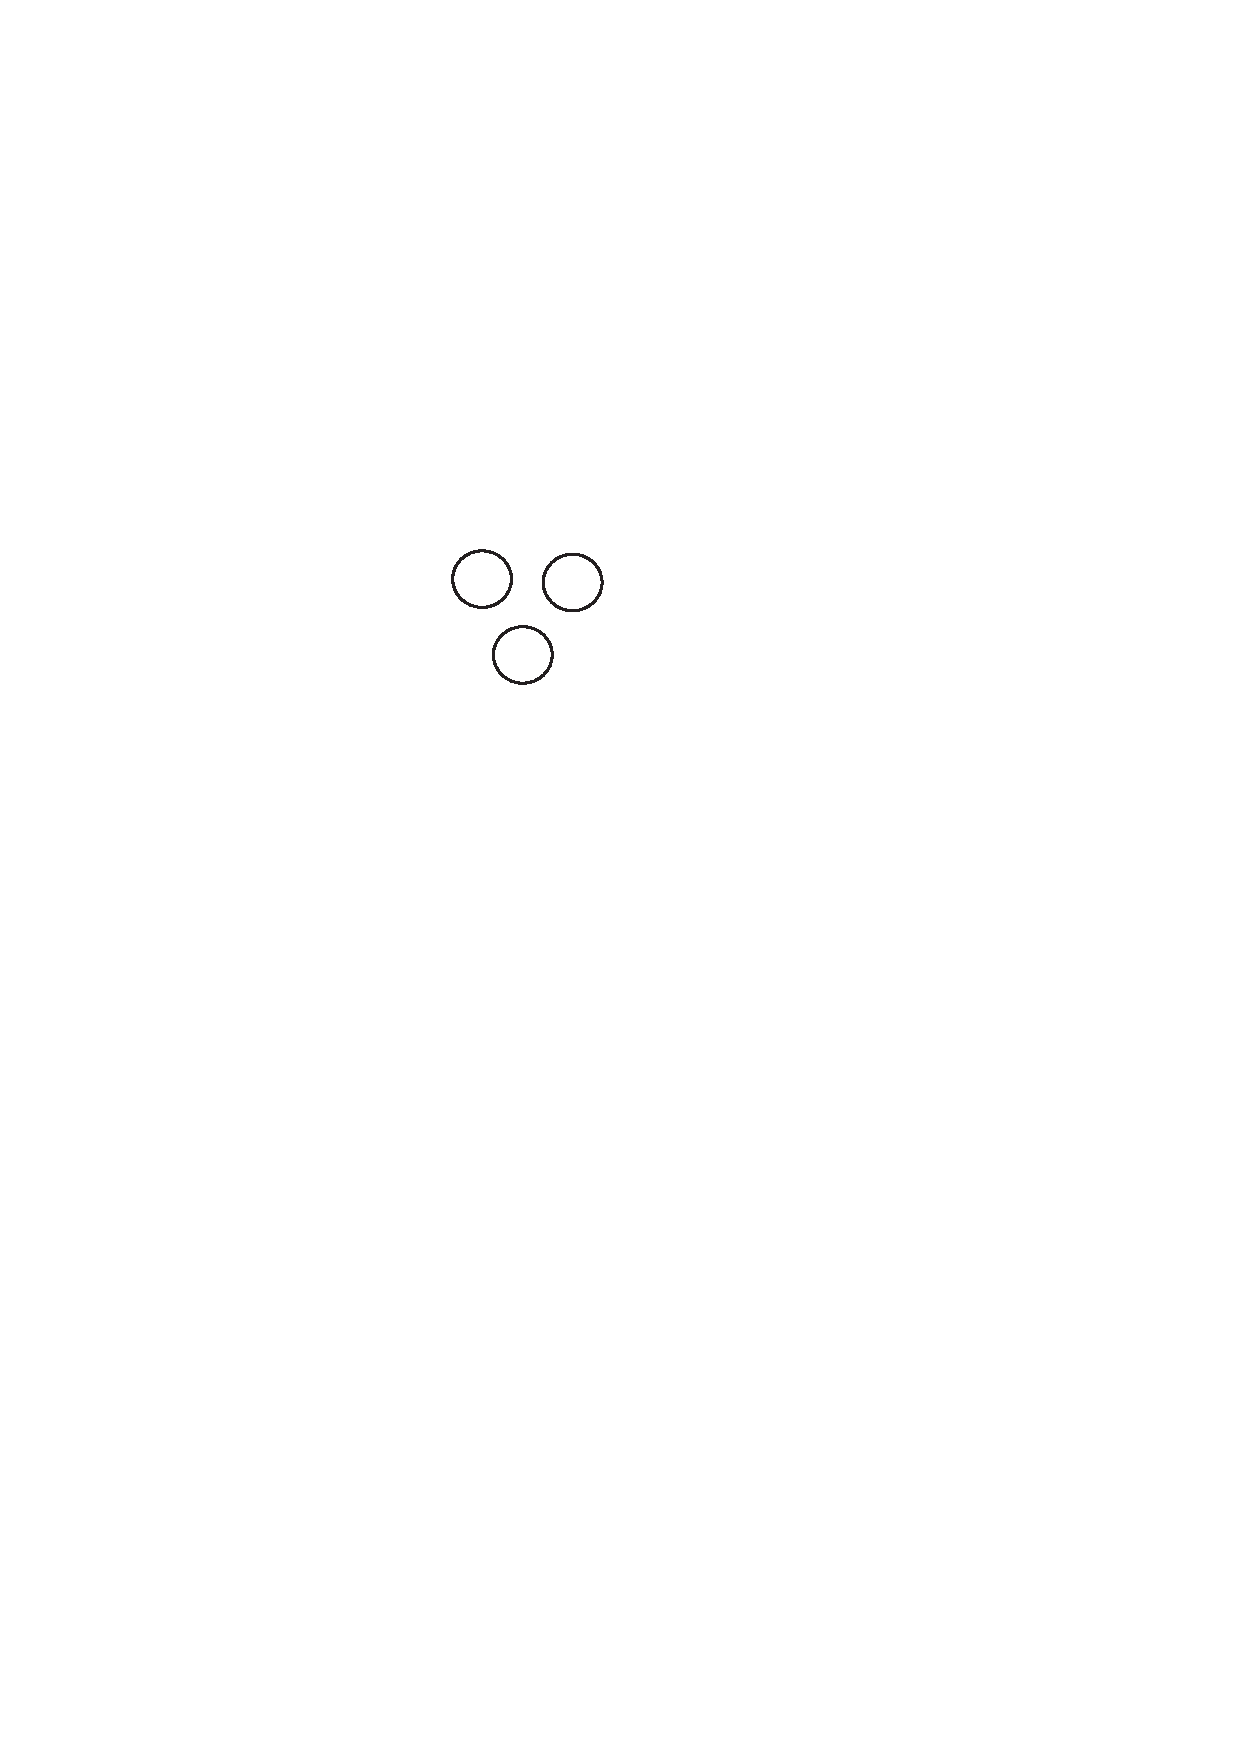
\includegraphics[width=0.02\textwidth]{images/oleum.pdf} & \"{O}l\\
$\smallfrown$ & Multiplikation\\
$\smallsmile$ & Division\\
$\bigtriangledown$ & Dreieck\\
\rule{1pt}{3mm} & K\"{u}rzung eines Bruchs\\
$f$ & facit\\
$\square$ \fbox{2} & Quadrat\\[0.5ex]
\fbox{3}~~cub. & Kubus\\[0.5ex]
$\surd~~~\sqrt{~~~}$ & Quadratwurzel\\
 =, aequ., aeq., $\sqcap$ & gleich\\
$\raisebox{0.8pt}{$\urcorner$} \hspace{-5.5pt}|\hspace{3pt}$ & gr\"{o}{\ss}er als\\
, ,, ,,, $\llcorner \lrcorner$ & Klammerausdr\"{u}cke\\
\ovalbox{\makebox[15mm][l]{~~~}} & Umrahmungen zur Bezeichnung wegfallender Terme\\
\leibdashv & Vorzeichen plus minus\\
\leibvdash & Vorzeichen minus plus\\
... & Platzhalter f\"{u}r Terme
\end{longtable}
